% ---------------------------------------------------------------
% Generated by Flowchart -> TikZ Studio
% Every coordinate below is derived from the editor diagram model.
% Safe to edit by hand, but regenerating will overwrite changes.
% ---------------------------------------------------------------

\documentclass[border=8pt]{standalone}
\usepackage[T1]{fontenc}
\usepackage[utf8]{inputenc}
\usepackage{xcolor}
\usepackage{tikz}
\usetikzlibrary{arrows.meta,shadows,shapes.geometric,shapes.misc}

% ---- Colour definitions ----
\definecolor{fc0F9B8E}{HTML}{0F9B8E}
\definecolor{fc12161C}{HTML}{12161C}
\definecolor{fc1F2933}{HTML}{1F2933}
\definecolor{fc2F6FEB}{HTML}{2F6FEB}
\definecolor{fc7C8A9B}{HTML}{7C8A9B}
\definecolor{fcC65B3C}{HTML}{C65B3C}
\definecolor{fcD4F0EA}{HTML}{D4F0EA}
\definecolor{fcDBE8FF}{HTML}{DBE8FF}
\definecolor{fcE6EDF4}{HTML}{E6EDF4}
\definecolor{fcF7F9FB}{HTML}{F7F9FB}
\definecolor{fcFADFD8}{HTML}{FADFD8}

% ---- Style definitions ----
\tikzset{
  fcnode/.style={
    draw, inner sep=0pt, outer sep=0pt, align=center,
    line join=round, line cap=butt
  },
  fcpath/.style={line join=round, line cap=butt},
  fcedge/.style={line join=round, line cap=butt},
  fclabel/.style={inner sep=1.4pt, outer sep=0pt, align=center},
}

\begin{document}
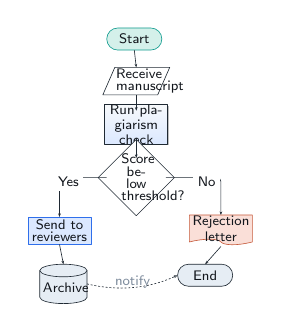
\begin{tikzpicture}[x=1cm, y=1cm]
  % ---- Nodes ----
  % n1 - Start / End "Start"
  \node[fcnode, shape=rounded rectangle, minimum width=0.7cm, minimum height=0.28cm,
        rounded rectangle arc length=180, draw=fc0F9B8E, line width=0.228pt, fill=fcD4F0EA,
        font=\fontsize{1.99pt}{2.49pt}\selectfont\sffamily, text=fc12161C, align=center,
        text width=0.532cm] (n1) at (1.65,-0.34) {Start};
  % n2 - Input / Output "Receive manuscript"
  \draw[fcpath, draw=fc1F2933, line width=0.228pt, fill=white]
    (1.403,-0.7) -- (2.1,-0.7) -- (1.947,-1.05) -- (1.25,-1.05) -- cycle;
  \coordinate (n2) at (1.675,-0.875);
  \node[fclabel, anchor=center, font=\fontsize{1.99pt}{2.49pt}\selectfont\sffamily,
        text=fc12161C, align=center, text width=0.51cm]
        at (1.675,-0.875) {Receive manuscript};
  % n3 - Process "Run plagiarism check"
  \node[fcnode, shape=rectangle, minimum width=0.8cm, minimum height=0.35cm, draw=fc1F2933,
        line width=0.228pt, top color=fcF7F9FB, bottom color=fcDBE8FF,
        drop shadow={shadow xshift=0.427pt, shadow yshift=-0.427pt, opacity=0.25, fill=black},
        font=\fontsize{1.99pt}{2.49pt}\selectfont\sffamily, text=fc12161C, align=center,
        text width=0.72cm] (n3) at (1.675,-1.425) {Run plagiarism check};
  % n4 - Decision "Score below"
  \node[fcnode, shape=diamond, minimum width=0.75cm, minimum height=0.5cm, draw=fc1F2933,
        line width=0.228pt, fill=white, font=\fontsize{1.99pt}{2.49pt}\selectfont\sffamily,
        text=fc12161C, align=center, text width=0.375cm]
        (n4) at (1.675,-2.1) {Score below \\ threshold?};
  % n5 - Process "Send to reviewers"
  \node[fcnode, shape=rectangle, minimum width=0.8cm, minimum height=0.35cm, draw=fc2F6FEB,
        line width=0.228pt, fill=fcDBE8FF, font=\fontsize{1.99pt}{2.49pt}\selectfont\sffamily,
        text=fc12161C, align=center, text width=0.72cm]
        (n5) at (0.7,-2.775) {Send to reviewers};
  % n6 - Document "Rejection letter"
  \draw[fcpath, draw=fcC65B3C, line width=0.228pt, fill=fcFADFD8]
    (2.35,-2.575) -- (3.15,-2.575) -- (3.15,-2.9174)
    .. controls (2.95,-2.9678) and (2.79,-2.9606) .. (2.75,-2.9174)
    .. controls (2.71,-2.8742) and (2.55,-2.867) .. (2.35,-2.9174) -- cycle;
  \coordinate (n6) at (2.75,-2.775);
  \node[fclabel, anchor=center, font=\fontsize{1.99pt}{2.49pt}\selectfont\sffamily,
        text=fc12161C, align=center, text width=0.72cm] at (2.75,-2.749) {Rejection letter};
  % n7 - Database "Archive"
  \draw[fcpath, draw=fc1F2933, line width=0.228pt, fill=fcE6EDF4]
    (0.45,-3.28) .. controls (0.45,-3.2358) and (0.5843,-3.2) .. (0.75,-3.2)
    .. controls (0.9157,-3.2) and (1.05,-3.2358) .. (1.05,-3.28) -- (1.05,-3.62)
    .. controls (1.05,-3.6642) and (0.9157,-3.7) .. (0.75,-3.7)
    .. controls (0.5843,-3.7) and (0.45,-3.6642) .. (0.45,-3.62) -- cycle;
  \draw[fcpath, draw=fc1F2933, line width=0.228pt]
    (0.45,-3.28) .. controls (0.45,-3.3242) and (0.5843,-3.36) .. (0.75,-3.36)
    .. controls (0.9157,-3.36) and (1.05,-3.3242) .. (1.05,-3.28);
  \coordinate (n7) at (0.75,-3.45);
  \node[fclabel, anchor=center, font=\fontsize{1.99pt}{2.49pt}\selectfont\sffamily,
        text=fc12161C, align=center, text width=0.52cm] at (0.75,-3.495) {Archive};
  % n8 - Start / End "End"
  \node[fcnode, shape=rounded rectangle, minimum width=0.7cm, minimum height=0.28cm,
        rounded rectangle arc length=180, draw=fc1F2933, line width=0.228pt, fill=fcE6EDF4,
        font=\fontsize{1.99pt}{2.49pt}\selectfont\sffamily, text=fc12161C, align=center,
        text width=0.532cm] (n8) at (2.55,-3.34) {End};
  % ---- Connectors ----
  % e1 - n1 -> n2 (straight)
  \draw[fcedge, -{Stealth[length=1.28pt, width=0.96pt]}, draw=fc1F2933, line width=0.228pt]
    (1.65,-0.48) -- (1.675,-0.7);
  % e2 - n2 -> n3 (straight)
  \draw[fcedge, -{Stealth[length=1.28pt, width=0.96pt]}, draw=fc1F2933, line width=0.228pt]
    (1.675,-1.05) -- (1.675,-1.25);
  % e3 - n3 -> n4 (straight)
  \draw[fcedge, -{Stealth[length=1.28pt, width=0.96pt]}, draw=fc1F2933, line width=0.228pt]
    (1.675,-1.6) -- (1.675,-1.85);
  % e4 - n4 -> n5 (rounded-orthogonal)
  \draw[fcedge, -{Stealth[length=1.28pt, width=0.96pt]}, draw=fc1F2933, line width=0.228pt]
    (1.3,-2.1) -- (1.24,-2.1) .. controls (1.2124,-2.1) and (1.1676,-2.1) .. (1.14,-2.1)
    -- (0.75,-2.1) .. controls (0.7224,-2.1) and (0.7,-2.1224) .. (0.7,-2.15) -- (0.7,-2.44)
    .. controls (0.7,-2.4676) and (0.7,-2.5124) .. (0.7,-2.54) -- (0.7,-2.6);
  \node[fclabel, anchor=center, font=\fontsize{1.71pt}{2.05pt}\selectfont\sffamily,
        text=fc12161C, fill=white, inner sep=1.6pt] (e4label) at (0.8147,-2.15) {Yes};
  % e5 - n4 -> n6 (rounded-orthogonal)
  \draw[fcedge, -{Stealth[length=1.28pt, width=0.96pt]}, draw=fc1F2933, line width=0.228pt]
    (2.05,-2.1) -- (2.11,-2.1) .. controls (2.1376,-2.1) and (2.1824,-2.1) .. (2.21,-2.1)
    -- (2.7,-2.1) .. controls (2.7276,-2.1) and (2.75,-2.1224) .. (2.75,-2.15)
    -- (2.75,-2.415) .. controls (2.75,-2.4426) and (2.75,-2.4874) .. (2.75,-2.515)
    -- (2.75,-2.575);
  \node[fclabel, anchor=center, font=\fontsize{1.71pt}{2.05pt}\selectfont\sffamily,
        text=fc12161C, fill=white, inner sep=1.6pt] (e5label) at (2.5691,-2.15) {No};
  % e6 - n5 -> n7 (straight)
  \draw[fcedge, -{Stealth[length=1.28pt, width=0.96pt]}, draw=fc1F2933, line width=0.228pt]
    (0.7,-2.95) -- (0.75,-3.2);
  % e7 - n6 -> n8 (straight)
  \draw[fcedge, -{Stealth[length=1.28pt, width=0.96pt]}, draw=fc1F2933, line width=0.228pt]
    (2.75,-2.975) -- (2.55,-3.2);
  % e8 - n7 -> n8 (curved)
  \draw[fcedge, -{Triangle[open, length=1.28pt, width=0.96pt]}, draw=fc1F2933,
        line width=0.228pt, dash pattern=on 0.683pt off 0.683pt]
    (1.05,-3.45) .. controls (1.446,-3.5461) and (1.8294,-3.5094) .. (2.2,-3.34);
  \node[fclabel, anchor=center, font=\fontsize{1.57pt}{1.88pt}\selectfont\sffamily,
        text=fc7C8A9B] (e8label) at (1.6279,-3.4249) {notify};
\end{tikzpicture}
\end{document}